\documentclass{standalone}
\usepackage{tikz}
\usetikzlibrary{patterns, positioning}

\begin{document}
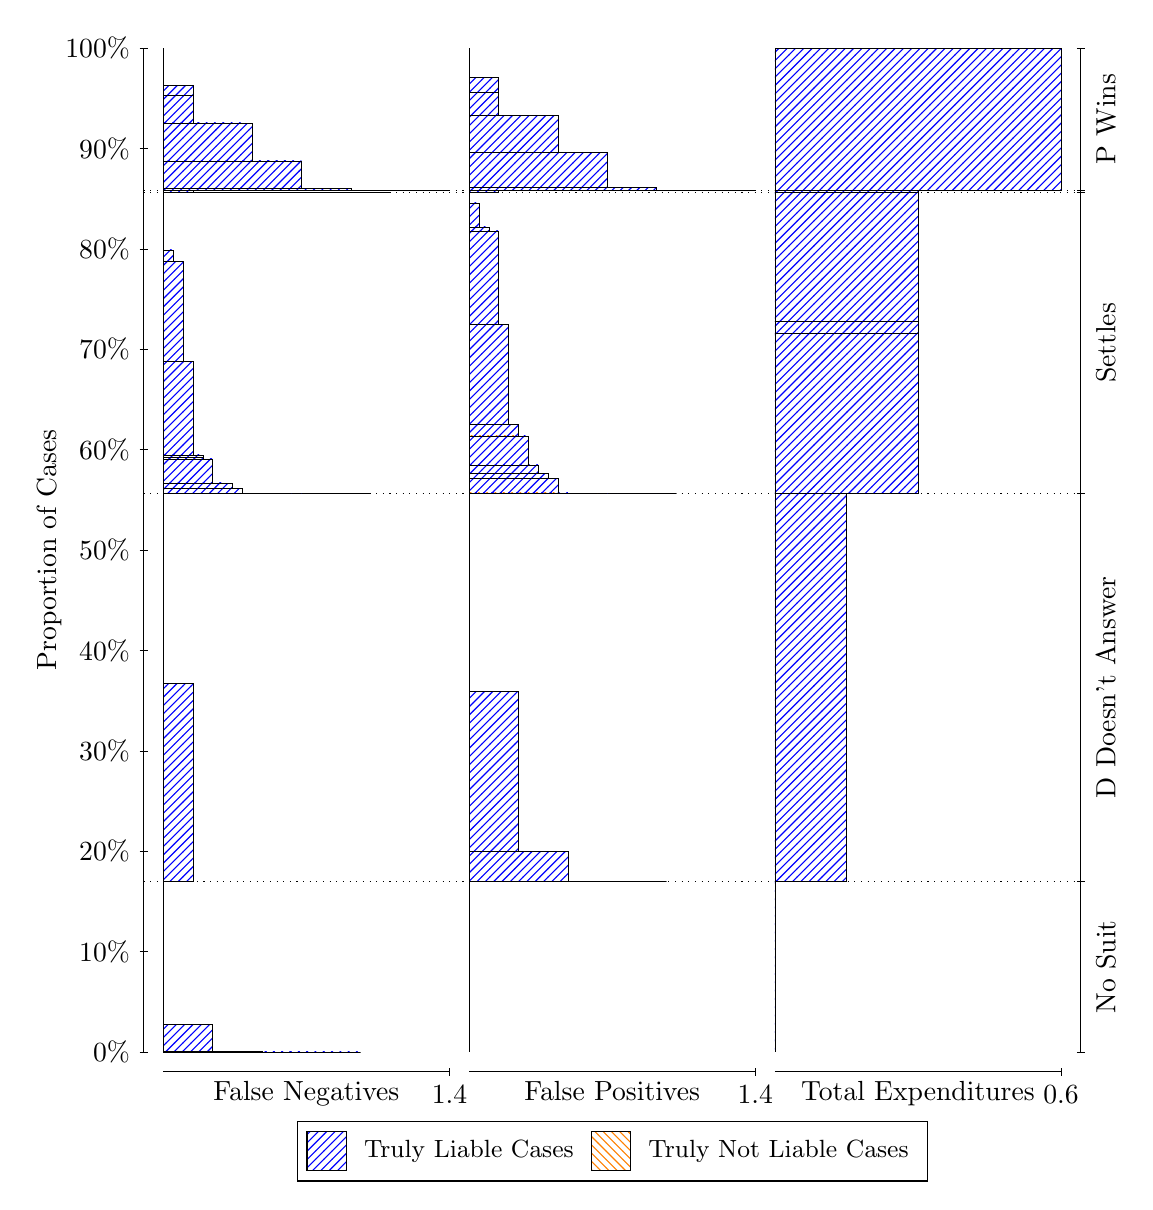
\begin{tikzpicture}
\draw[black, very thin] (1.5,1.75) -- (1.5,14.5);
\node[rotate=90, anchor=center] at (0.3, 8.125) {Proportion of Cases};
\draw[black, very thin] (1.45,1.75) -- (1.55,1.75);
\node[anchor=east] at (1.45, 1.75) {0\%};
\draw[black, very thin] (1.45,3.025) -- (1.55,3.025);
\node[anchor=east] at (1.45, 3.025) {10\%};
\draw[black, very thin] (1.45,4.3) -- (1.55,4.3);
\node[anchor=east] at (1.45, 4.3) {20\%};
\draw[black, very thin] (1.45,5.575) -- (1.55,5.575);
\node[anchor=east] at (1.45, 5.575) {30\%};
\draw[black, very thin] (1.45,6.85) -- (1.55,6.85);
\node[anchor=east] at (1.45, 6.85) {40\%};
\draw[black, very thin] (1.45,8.125) -- (1.55,8.125);
\node[anchor=east] at (1.45, 8.125) {50\%};
\draw[black, very thin] (1.45,9.4) -- (1.55,9.4);
\node[anchor=east] at (1.45, 9.4) {60\%};
\draw[black, very thin] (1.45,10.675) -- (1.55,10.675);
\node[anchor=east] at (1.45, 10.675) {70\%};
\draw[black, very thin] (1.45,11.95) -- (1.55,11.95);
\node[anchor=east] at (1.45, 11.95) {80\%};
\draw[black, very thin] (1.45,13.225) -- (1.55,13.225);
\node[anchor=east] at (1.45, 13.225) {90\%};
\draw[black, very thin] (1.45,14.5) -- (1.55,14.5);
\node[anchor=east] at (1.45, 14.5) {100\%};

\draw[black, very thin] (13.4,1.75) -- (13.4,14.5);
\draw[black, very thin] (13.35,1.75) -- (13.45,1.75);
\node[anchor=west] at (13.35, 1.75) {};
\draw[black, very thin] (13.35,3.9148) -- (13.45,3.9148);
\node[anchor=west] at (13.35, 3.9148) {};
\draw[black, very thin] (13.35,8.844) -- (13.45,8.844);
\node[anchor=west] at (13.35, 8.844) {};
\draw[black, very thin] (13.35,12.667) -- (13.45,12.667);
\node[anchor=west] at (13.35, 12.667) {};
\draw[black, very thin] (13.35,12.695) -- (13.45,12.695);
\node[anchor=west] at (13.35, 12.695) {};
\draw[black, very thin] (13.35,14.5) -- (13.45,14.5);
\node[anchor=west] at (13.35, 14.5) {};

\draw[black, very thin, pattern color=blue, pattern=north east lines] (1.75,1.75) rectangle (4.2557,1.75);
\draw[black, very thin, pattern color=blue, pattern=north east lines] (1.75,1.75) rectangle (3.6293,1.75);
\draw[black, very thin, pattern color=blue, pattern=north east lines] (1.75,1.75) rectangle (3.0029,1.753);
\draw[black, very thin, pattern color=blue, pattern=north east lines] (1.75,1.753) rectangle (2.3764,2.1045);
\draw[black, very thin, pattern color=orange, pattern=north west lines] (1.75,2.1045) rectangle (1.75,2.1045);
\draw[black, very thin, pattern color=blue, pattern=north east lines] (1.75,2.1045) rectangle (1.75,3.9148);
\draw[black, very thin, pattern color=blue, pattern=north east lines] (1.75,3.9148) rectangle (2.1259,6.43);
\draw[black, very thin, pattern color=orange, pattern=north west lines] (1.75,6.43) rectangle (1.75,6.43);
\draw[black, very thin, pattern color=blue, pattern=north east lines] (1.75,6.43) rectangle (1.75,8.844);
\draw[black, very thin, pattern color=blue, pattern=north east lines] (1.75,8.844) rectangle (4.381,8.844);
\draw[black, very thin, pattern color=blue, pattern=north east lines] (1.75,8.844) rectangle (4.1305,8.844);
\draw[black, very thin, pattern color=blue, pattern=north east lines] (1.75,8.844) rectangle (3.8799,8.844);
\draw[black, very thin, pattern color=blue, pattern=north east lines] (1.75,8.844) rectangle (3.7546,8.844);
\draw[black, very thin, pattern color=blue, pattern=north east lines] (1.75,8.844) rectangle (3.6293,8.844);
\draw[black, very thin, pattern color=blue, pattern=north east lines] (1.75,8.844) rectangle (3.504,8.844);
\draw[black, very thin, pattern color=blue, pattern=north east lines] (1.75,8.844) rectangle (3.3787,8.844);
\draw[black, very thin, pattern color=blue, pattern=north east lines] (1.75,8.844) rectangle (3.2534,8.844);
\draw[black, very thin, pattern color=blue, pattern=north east lines] (1.75,8.844) rectangle (3.1282,8.844);
\draw[black, very thin, pattern color=blue, pattern=north east lines] (1.75,8.844) rectangle (3.0029,8.8445);
\draw[black, very thin, pattern color=blue, pattern=north east lines] (1.75,8.8445) rectangle (2.8776,8.8446);
\draw[black, very thin, pattern color=blue, pattern=north east lines] (1.75,8.8446) rectangle (2.8776,8.8447);
\draw[black, very thin, pattern color=blue, pattern=north east lines] (1.75,8.8447) rectangle (2.7523,8.9088);
\draw[black, very thin, pattern color=blue, pattern=north east lines] (1.75,8.9088) rectangle (2.627,8.9723);
\draw[black, very thin, pattern color=blue, pattern=north east lines] (1.75,8.9723) rectangle (2.5017,8.9724);
\draw[black, very thin, pattern color=blue, pattern=north east lines] (1.75,8.9724) rectangle (2.5017,8.9778);
\draw[black, very thin, pattern color=blue, pattern=north east lines] (1.75,8.9778) rectangle (2.3764,9.2822);
\draw[black, very thin, pattern color=blue, pattern=north east lines] (1.75,9.2822) rectangle (2.2511,9.3001);
\draw[black, very thin, pattern color=blue, pattern=north east lines] (1.75,9.3001) rectangle (2.2511,9.3326);
\draw[black, very thin, pattern color=blue, pattern=north east lines] (1.75,9.3326) rectangle (2.1259,10.522);
\draw[black, very thin, pattern color=blue, pattern=north east lines] (1.75,10.522) rectangle (2.0006,11.789);
\draw[black, very thin, pattern color=blue, pattern=north east lines] (1.75,11.789) rectangle (2.0006,11.789);
\draw[black, very thin, pattern color=blue, pattern=north east lines] (1.75,11.789) rectangle (1.8753,11.793);
\draw[black, very thin, pattern color=blue, pattern=north east lines] (1.75,11.793) rectangle (1.8753,11.935);
\draw[black, very thin, pattern color=orange, pattern=north west lines] (1.75,11.935) rectangle (1.75,11.935);
\draw[black, very thin, pattern color=blue, pattern=north east lines] (1.75,11.935) rectangle (1.75,12.667);
\draw[black, very thin, pattern color=blue, pattern=north east lines] (1.75,12.667) rectangle (4.6316,12.667);
\draw[black, very thin, pattern color=blue, pattern=north east lines] (1.75,12.667) rectangle (4.0052,12.667);
\draw[black, very thin, pattern color=blue, pattern=north east lines] (1.75,12.667) rectangle (3.3787,12.667);
\draw[black, very thin, pattern color=blue, pattern=north east lines] (1.75,12.667) rectangle (2.7523,12.671);
\draw[black, very thin, pattern color=blue, pattern=north east lines] (1.75,12.671) rectangle (2.1259,12.695);
\draw[black, very thin, pattern color=orange, pattern=north west lines] (1.75,12.695) rectangle (1.75,12.695);
\draw[black, very thin, pattern color=blue, pattern=north east lines] (1.75,12.695) rectangle (5.3833,12.695);
\draw[black, very thin, pattern color=blue, pattern=north east lines] (1.75,12.695) rectangle (4.7569,12.695);
\draw[black, very thin, pattern color=blue, pattern=north east lines] (1.75,12.695) rectangle (4.1305,12.717);
\draw[black, very thin, pattern color=blue, pattern=north east lines] (1.75,12.717) rectangle (4.0052,12.717);
\draw[black, very thin, pattern color=blue, pattern=north east lines] (1.75,12.717) rectangle (3.504,13.066);
\draw[black, very thin, pattern color=blue, pattern=north east lines] (1.75,13.066) rectangle (3.3787,13.066);
\draw[black, very thin, pattern color=blue, pattern=north east lines] (1.75,13.066) rectangle (2.8776,13.547);
\draw[black, very thin, pattern color=blue, pattern=north east lines] (1.75,13.547) rectangle (2.7523,13.55);
\draw[black, very thin, pattern color=blue, pattern=north east lines] (1.75,13.55) rectangle (2.2511,13.55);
\draw[black, very thin, pattern color=blue, pattern=north east lines] (1.75,13.55) rectangle (2.1259,13.894);
\draw[black, very thin, pattern color=blue, pattern=north east lines] (1.75,13.894) rectangle (2.1259,14.023);
\draw[black, very thin, pattern color=orange, pattern=north west lines] (1.75,14.023) rectangle (1.75,14.023);
\draw[black, very thin, pattern color=blue, pattern=north east lines] (1.75,14.023) rectangle (1.75,14.5);
\draw[black, very thin, pattern color=orange, pattern=north west lines] (5.6333,1.75) rectangle (5.6333,1.75);
\draw[black, very thin, pattern color=blue, pattern=north east lines] (5.6333,1.75) rectangle (5.6333,3.9148);
\draw[black, very thin, pattern color=orange, pattern=north west lines] (5.6333,3.9148) rectangle (8.1391,3.9148);
\draw[black, very thin, pattern color=blue, pattern=north east lines] (5.6333,3.9148) rectangle (8.1391,3.9148);
\draw[black, very thin, pattern color=blue, pattern=north east lines] (5.6333,3.9148) rectangle (7.5126,3.9176);
\draw[black, very thin, pattern color=blue, pattern=north east lines] (5.6333,3.9176) rectangle (6.8862,4.2959);
\draw[black, very thin, pattern color=blue, pattern=north east lines] (5.6333,4.2959) rectangle (6.2598,6.3288);
\draw[black, very thin, pattern color=blue, pattern=north east lines] (5.6333,6.3288) rectangle (5.6333,8.844);
\draw[black, very thin, pattern color=orange, pattern=north west lines] (5.6333,8.844) rectangle (8.2644,8.844);
\draw[black, very thin, pattern color=blue, pattern=north east lines] (5.6333,8.844) rectangle (8.2644,8.844);
\draw[black, very thin, pattern color=orange, pattern=north west lines] (5.6333,8.844) rectangle (8.0138,8.844);
\draw[black, very thin, pattern color=blue, pattern=north east lines] (5.6333,8.844) rectangle (8.0138,8.844);
\draw[black, very thin, pattern color=orange, pattern=north west lines] (5.6333,8.844) rectangle (7.7632,8.844);
\draw[black, very thin, pattern color=blue, pattern=north east lines] (5.6333,8.844) rectangle (7.7632,8.844);
\draw[black, very thin, pattern color=blue, pattern=north east lines] (5.6333,8.844) rectangle (7.6379,8.844);
\draw[black, very thin, pattern color=orange, pattern=north west lines] (5.6333,8.844) rectangle (7.5126,8.844);
\draw[black, very thin, pattern color=blue, pattern=north east lines] (5.6333,8.844) rectangle (7.5126,8.844);
\draw[black, very thin, pattern color=blue, pattern=north east lines] (5.6333,8.844) rectangle (7.3874,8.844);
\draw[black, very thin, pattern color=orange, pattern=north west lines] (5.6333,8.844) rectangle (7.2621,8.844);
\draw[black, very thin, pattern color=blue, pattern=north east lines] (5.6333,8.844) rectangle (7.2621,8.844);
\draw[black, very thin, pattern color=blue, pattern=north east lines] (5.6333,8.844) rectangle (7.1368,8.844);
\draw[black, very thin, pattern color=orange, pattern=north west lines] (5.6333,8.844) rectangle (7.0115,8.844);
\draw[black, very thin, pattern color=blue, pattern=north east lines] (5.6333,8.844) rectangle (7.0115,8.8489);
\draw[black, very thin, pattern color=blue, pattern=north east lines] (5.6333,8.8489) rectangle (6.8862,8.849);
\draw[black, very thin, pattern color=blue, pattern=north east lines] (5.6333,8.849) rectangle (6.7609,8.849);
\draw[black, very thin, pattern color=orange, pattern=north west lines] (5.6333,8.849) rectangle (6.7609,8.849);
\draw[black, very thin, pattern color=blue, pattern=north east lines] (5.6333,8.849) rectangle (6.7609,9.036);
\draw[black, very thin, pattern color=blue, pattern=north east lines] (5.6333,9.036) rectangle (6.6356,9.0995);
\draw[black, very thin, pattern color=orange, pattern=north west lines] (5.6333,9.0995) rectangle (6.5103,9.0995);
\draw[black, very thin, pattern color=blue, pattern=north east lines] (5.6333,9.0995) rectangle (6.5103,9.2067);
\draw[black, very thin, pattern color=blue, pattern=north east lines] (5.6333,9.2067) rectangle (6.3851,9.5755);
\draw[black, very thin, pattern color=orange, pattern=north west lines] (5.6333,9.5755) rectangle (6.2598,9.5755);
\draw[black, very thin, pattern color=blue, pattern=north east lines] (5.6333,9.5755) rectangle (6.2598,9.7215);
\draw[black, very thin, pattern color=blue, pattern=north east lines] (5.6333,9.7215) rectangle (6.1345,9.7215);
\draw[black, very thin, pattern color=blue, pattern=north east lines] (5.6333,9.7215) rectangle (6.1345,10.989);
\draw[black, very thin, pattern color=blue, pattern=north east lines] (5.6333,10.989) rectangle (6.0092,12.178);
\draw[black, very thin, pattern color=blue, pattern=north east lines] (5.6333,12.178) rectangle (5.8839,12.228);
\draw[black, very thin, pattern color=blue, pattern=north east lines] (5.6333,12.228) rectangle (5.7586,12.533);
\draw[black, very thin, pattern color=blue, pattern=north east lines] (5.6333,12.533) rectangle (5.6333,12.667);
\draw[black, very thin, pattern color=orange, pattern=north west lines] (5.6333,12.667) rectangle (6.0092,12.667);
\draw[black, very thin, pattern color=blue, pattern=north east lines] (5.6333,12.667) rectangle (6.0092,12.691);
\draw[black, very thin, pattern color=blue, pattern=north east lines] (5.6333,12.691) rectangle (5.6333,12.695);
\draw[black, very thin, pattern color=orange, pattern=north west lines] (5.6333,12.695) rectangle (9.2667,12.695);
\draw[black, very thin, pattern color=blue, pattern=north east lines] (5.6333,12.695) rectangle (9.2667,12.695);
\draw[black, very thin, pattern color=orange, pattern=north west lines] (5.6333,12.695) rectangle (8.6402,12.695);
\draw[black, very thin, pattern color=blue, pattern=north east lines] (5.6333,12.695) rectangle (8.6402,12.695);
\draw[black, very thin, pattern color=orange, pattern=north west lines] (5.6333,12.695) rectangle (8.0138,12.695);
\draw[black, very thin, pattern color=blue, pattern=north east lines] (5.6333,12.695) rectangle (8.0138,12.73);
\draw[black, very thin, pattern color=orange, pattern=north west lines] (5.6333,12.73) rectangle (7.3874,12.73);
\draw[black, very thin, pattern color=blue, pattern=north east lines] (5.6333,12.73) rectangle (7.3874,13.171);
\draw[black, very thin, pattern color=orange, pattern=north west lines] (5.6333,13.171) rectangle (7.2621,13.171);
\draw[black, very thin, pattern color=blue, pattern=north east lines] (5.6333,13.171) rectangle (7.2621,13.171);
\draw[black, very thin, pattern color=blue, pattern=north east lines] (5.6333,13.171) rectangle (6.7609,13.645);
\draw[black, very thin, pattern color=orange, pattern=north west lines] (5.6333,13.645) rectangle (6.6356,13.645);
\draw[black, very thin, pattern color=blue, pattern=north east lines] (5.6333,13.645) rectangle (6.6356,13.645);
\draw[black, very thin, pattern color=blue, pattern=north east lines] (5.6333,13.645) rectangle (6.1345,13.648);
\draw[black, very thin, pattern color=blue, pattern=north east lines] (5.6333,13.648) rectangle (6.0092,13.933);
\draw[black, very thin, pattern color=orange, pattern=north west lines] (5.6333,13.933) rectangle (6.0092,13.933);
\draw[black, very thin, pattern color=blue, pattern=north east lines] (5.6333,13.933) rectangle (6.0092,14.129);
\draw[black, very thin, pattern color=blue, pattern=north east lines] (5.6333,14.129) rectangle (5.6333,14.5);
\draw[black, very thin, pattern color=orange, pattern=north west lines] (9.5167,1.75) rectangle (9.5167,1.75);
\draw[black, very thin, pattern color=blue, pattern=north east lines] (9.5167,1.75) rectangle (9.5167,3.9148);
\draw[black, very thin, pattern color=orange, pattern=north west lines] (9.5167,3.9148) rectangle (10.425,3.9148);
\draw[black, very thin, pattern color=blue, pattern=north east lines] (9.5167,3.9148) rectangle (10.425,8.844);
\draw[black, very thin, pattern color=orange, pattern=north west lines] (9.5167,8.844) rectangle (11.333,8.844);
\draw[black, very thin, pattern color=blue, pattern=north east lines] (9.5167,8.844) rectangle (11.333,10.88);
\draw[black, very thin, pattern color=orange, pattern=north west lines] (9.5167,10.88) rectangle (11.333,10.88);
\draw[black, very thin, pattern color=blue, pattern=north east lines] (9.5167,10.88) rectangle (11.333,11.027);
\draw[black, very thin, pattern color=orange, pattern=north west lines] (9.5167,11.027) rectangle (11.333,11.027);
\draw[black, very thin, pattern color=blue, pattern=north east lines] (9.5167,11.027) rectangle (11.333,12.667);
\draw[black, very thin, pattern color=orange, pattern=north west lines] (9.5167,12.667) rectangle (11.333,12.667);
\draw[black, very thin, pattern color=blue, pattern=north east lines] (9.5167,12.667) rectangle (11.333,12.695);
\draw[black, very thin, pattern color=orange, pattern=north west lines] (9.5167,12.695) rectangle (13.15,12.695);
\draw[black, very thin, pattern color=blue, pattern=north east lines] (9.5167,12.695) rectangle (13.15,14.5);
\draw[black, dotted] (1.5,3.9148) -- (13.4,3.9148);
\draw[black, dotted] (1.5,8.844) -- (13.4,8.844);
\draw[black, dotted] (1.5,12.667) -- (13.4,12.667);
\draw[black, dotted] (1.5,12.695) -- (13.4,12.695);
\draw[black, very thin] (1.75,1.5) -- (5.3833,1.5);
\node[anchor=north] at (3.5667, 1.5) {False Negatives};
\draw[black, very thin] (5.3833,1.45) -- (5.3833,1.55);
\node[anchor=north] at (5.3833, 1.45) {1.4};

\draw[black, very thin] (5.6333,1.5) -- (9.2667,1.5);
\node[anchor=north] at (7.45, 1.5) {False Positives};
\draw[black, very thin] (9.2667,1.45) -- (9.2667,1.55);
\node[anchor=north] at (9.2667, 1.45) {1.4};

\draw[black, very thin] (9.5167,1.5) -- (13.15,1.5);
\node[anchor=north] at (11.333, 1.5) {Total Expenditures};
\draw[black, very thin] (13.15,1.45) -- (13.15,1.55);
\node[anchor=north] at (13.15, 1.45) {0.6};

\node[black, centered, rotate=90] at (13.72, 2.8324) {No Suit};
\node[black, centered, rotate=90] at (13.72, 6.3794) {D Doesn't Answer};
\node[black, centered, rotate=90] at (13.72, 10.755) {Settles};

\node[black, centered, rotate=90] at (13.72, 13.597) {P Wins};

\draw (7.449999999999999,1.5) node[draw=none] (baseCoordinate) {};
\begin{scope}[align=center]
        \matrix[scale=0.5, draw=black, below=0.5cm of baseCoordinate, nodes={draw}, column sep=0.1cm]{
            \node[rectangle, draw, minimum width=0.5cm, minimum height=0.5cm, pattern=north east lines, pattern color=blue] {}; &
            \node[draw=none, font=\small] (B) {Truly Liable Cases}; &
            \node[rectangle, draw, minimum width=0.5cm, minimum height=0.5cm, pattern=north west lines, pattern color=orange] {}; &
            \node[draw=none, font=\small] (B) {Truly Not Liable Cases}; \\
            };
\end{scope}

\end{tikzpicture}
\end{document}